\documentclass{article}

\usepackage{graphicx}
\usepackage{tikz}
\usepackage{tikzsymbols}
\usetikzlibrary{calc,patterns,shapes.geometric}
\pagestyle{empty}
\usepackage[margin=0pt]{geometry}
\geometry{papersize={14in,12in}}

\def\centerarc[#1](#2)(#3:#4:#5){\draw[#1] ($(#2)+({#5*cos(#3)},{#5*sin(#3)})$) arc (#3:#4:#5);}

\begin{document}
	\begin{figure}
		\centering
		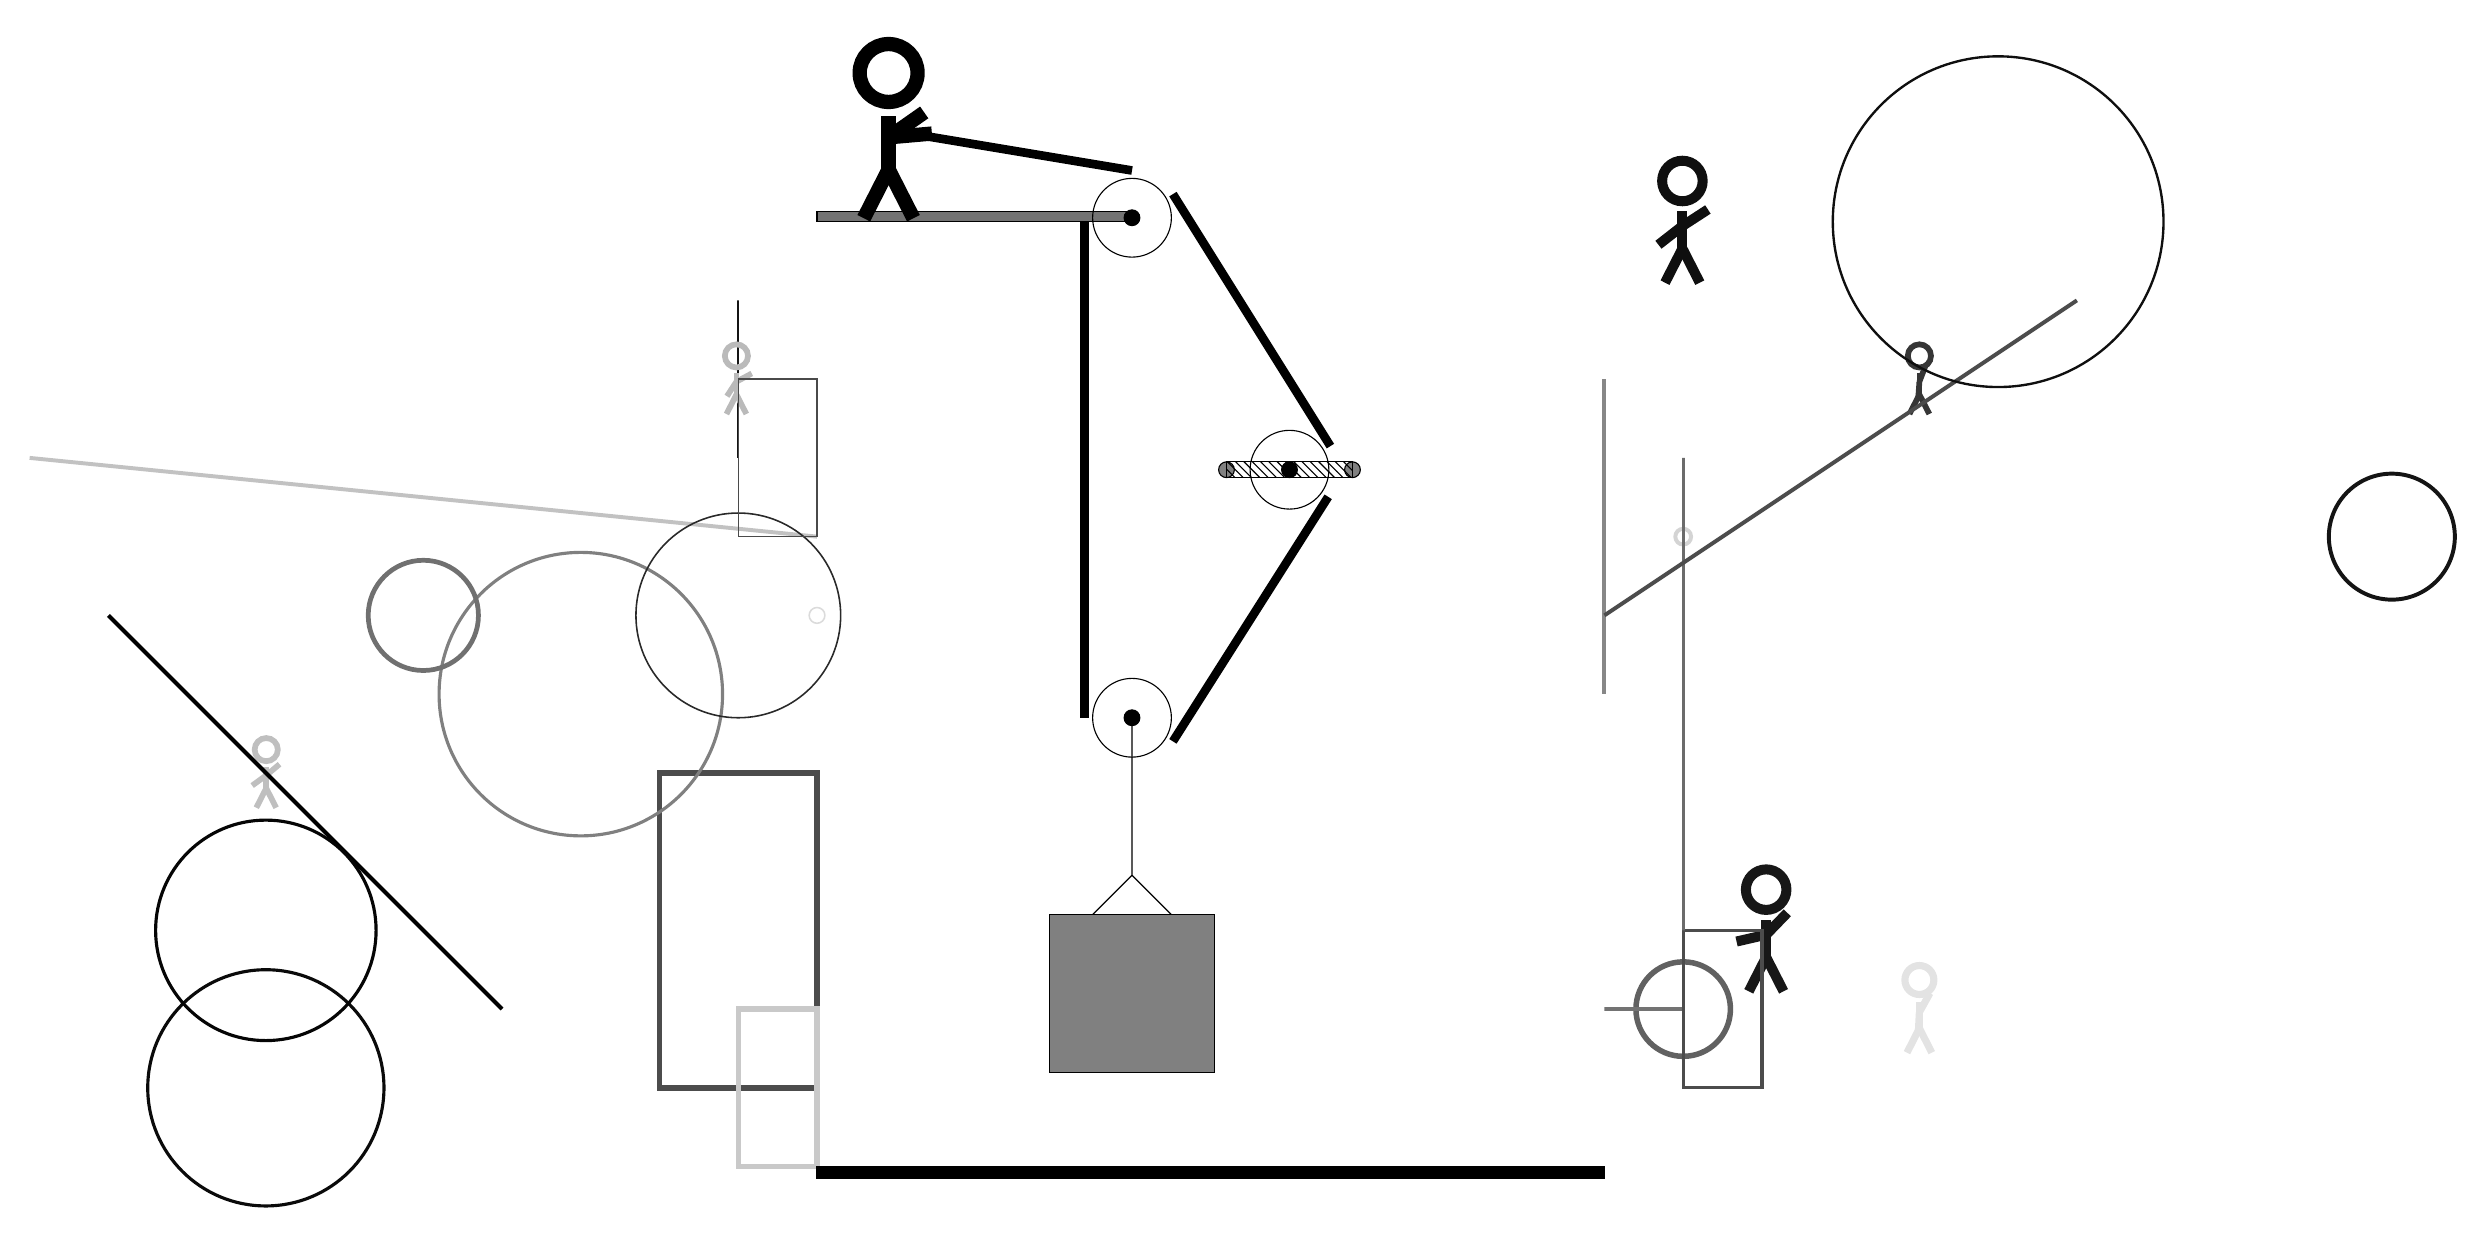
\begin{tikzpicture}
			%%%%% START %%%%%
			
			\draw[fill=black!55] (-2, 9) rectangle (2, 9.125);
			
			\draw (2, 2.7) circle (0.5);
			\draw[fill=black] (2, 2.7) circle (0.1);
			
			\draw (2, 9.05) circle (0.5);
			\draw[fill=black] (2, 9.05) circle (0.1);
			
			\draw[fill=white](4, 5.85) circle (0.5);
			\draw[fill=black] (4, 5.85) circle (0.1);
			\draw[fill=black!50] (3.2, 5.85) circle (0.1);
			\draw[fill=black!50] (4.8, 5.85) circle (0.1);
			\draw[pattern=north west lines, pattern color=black] (3.2, 5.95) rectangle (4.8, 5.75);
			
			\draw (2, 2.7) -- (2, 0.7) -- (1.5, 0.2) -- (2.5, 0.2) -- (2, 0.7);
			\draw[fill=black!50] (0.95, 0.2) rectangle (3.05, -1.8);
			
			\draw[line width=1.1mm] (1.4, 9) -- (1.4, 2.7);
			\centerarc[line width=1.1mm](2, 2.7)(180:330:0.6);
			\draw[line width=1.1mm](2.5196, 2.4) -- (4.4915, 5.5058);
			\centerarc[line width=1.1mm](4, 5.85)(390:325:0.6);
			\draw[line width=1.1mm](4.5196, 6.15) -- (2.5196, 9.35);
			\centerarc[line width=1.1mm](2, 9.05)(30:90:0.6);
			\draw[line width=1.1mm](2, 9.65) -- (-1, 10.15);
			
			\draw [line width=0.4mm, color=black!96](-9, -2) circle (1.5);
			
			\draw[line width=0.5mm, color=black!24](-2, 5) -- (-12, 6);
			\draw[line width=0.7mm, color=black!70] (-2, -2) rectangle (-4, 2);
			\node[line width=0.2mm, color=black!91] at (10, 0) {\Strichmaxerl[7][13][46]};
			\draw [line width=0.7mm, color=black!62](9, -1) circle (0.6);
			
			\draw[line width=0.5mm, color=black!47](8, 7) -- (8, 3);
			\draw [line width=0.4mm, color=black!50](-5, 3) circle (1.8);
			
			\node[line width=0.3mm, color=black!25] at (-9, 2) {\Strichmaxerl[4][36][40]};
			\draw[line width=0.5mm, color=black!100](-6, -1) -- (-11, 4);
			\draw[line width=0.5mm, color=black!55] (8, -1) rectangle (9, -1);
			\draw[line width=0.3mm, color=black!92] (-3, 6) rectangle (-3, 8);
			\draw [line width=0.5mm, color=black!17](9, 5) circle (0.1);
			\draw[line width=0.4mm, color=black!70] (10, 0) rectangle (9, -2);
			\node[line width=0.6mm, color=black!79] at (12, 7) {\Strichmaxerl[4][86][69]};
			\node[line width=0.2mm, color=black!11] at (12, -1) {\Strichmaxerl[5][87][61]};
			\draw [line width=0.2mm, color=black!84](-3, 4) circle (1.3);
			\draw[line width=0.4mm, color=black!58] (9, 0) rectangle (9, 6);
			
			\draw[line width=0.7mm, color=black!21] (-3, -1) rectangle (-2, -3);
			\draw[line width=0.5mm, color=black!70](8, 4) -- (14, 8);
			\draw [line width=0.4mm, color=black!98](-9, 0) circle (1.4);
			\node[line width=0.7mm, color=black!27] at (-3, 7) {\Strichmaxerl[4][57][28]};
			\draw [line width=0.3mm, color=black!94](13, 9) circle (2.1);
			\draw[line width=0.2mm, color=black!71] (-3, 5) rectangle (-2, 7);
			\draw [line width=0.5mm, color=black!92](18, 5) circle (0.8);
			\draw [line width=0.2mm, color=black!14](-2, 4) circle (0.1);
			
			\node[line width=0.5mm, color=black!94] at (9, 9) {\Strichmaxerl[7][38][33]};
			\draw [line width=0.6mm, color=black!56](-7, 4) circle (0.7);
			
			\node at (-1, 10.15) {\Strichmaxerl[10][-175][35]};
			
			\draw[fill=black] (-2, -3) rectangle (8, -3.15);
			
			%%%%% END %%%%%
		\end{tikzpicture}
	\end{figure}	
\end{document}